% プロジェクト学習中間報告書書式テンプレート ver.1.0 (iso-2022-jp)

% 両面印刷する場合は `openany' を削除する
\documentclass[openany,11pt,papersize]{jsbook}



% 報告書提出用スタイルファイル
%\usepackage[final]{funpro}%最終報告書
\usepackage[middle]{funpro}%中間報告書

% 画像ファイル (EPS, EPDF, PNG) を読み込むために
\usepackage[dvipdfmx]{graphicx,color}

% ここから -->
\usepackage{calc,ifthen}
\newcounter{hoge}
\newcommand{\fake}[1]{\whiledo{\thehoge<70}{#1\stepcounter{hoge}}%
  \setcounter{hoge}{0}}
% <-- ここまで 削除してもよい

% 年度の指定
\thisYear{2015}

% プロジェクト名
\jProjectName{フィールドから創る地域・社会のためのスウィフトなアプリ開発}

% [簡易版のプロジェクト名]{正式なプロジェクト名}
% 欧文のプロジェクト名が極端に長い(2行を超える)場合は、短い記述を
% 任意引数として渡す。
%\eProjectName[Making Delicious curry]{How to make delicious curry of Hakodate}
\eProjectName{``Swift'' Application Development Based on Field Research}


% <プロジェクト番号>-<グループ名>
\ProjectNumber{3-A}

% グループ名
\jGroupName{観光系グループ}
\eGroupName{Tourism Group}

% プロジェクトリーダ
\ProjectLeader{1013220}{新保遥平}{Yohei~Shinpo}

% グループリーダ
\GroupLeader  {1013068}{岩見建汰}{Kenta~Iwami}

% メンバー数
\SumOfMembers{5}
% グループメンバ
\GroupMember  {1}{1013001}{池田俊輝}{Toshiki~Ikeda}
\GroupMember  {2}{1013068}{岩見建汰}{Kenta~Iwami}
\GroupMember  {3}{1013167}{山川拓也}{Takuya~Yamakawa}
\GroupMember  {4}{1013224}{細川椋太}{Ryota~Hosokawa}
\GroupMember  {5}{1013228}{横山翔栄}{Shoei~Yokoyama}

% 指導教員
\jadvisor{伊藤恵,奥野拓,原田泰,木塚あゆみ,南部美砂子}
% 複数人数いる場合はカンマ(,)で区切る。カンマの前後に空白は入れない。
\eadvisor{Kei~Itou,Taku~Okuno,Yasushi~Harada,Ayumi~Kizuka,Misako~Nambu}

% 論文提出日
\jdate{2015年7月29日}
\edate{July~29, 2015}

\begin{document}
%
% 表紙
\maketitle

%前付け
\frontmatter

% 和文
\begin{jabstract}
\quad 本プロジェクトでは、まずフィールドを実際に調査してそこから問題点を見つける。そこで見つかった問題点を解決するためにiOSアプリケーション(以下、アプリとする)を開発して、それにより地域・社会に貢献することを目標として活動を行っている。開発手法はアジャイル開発を用いる。素早くアプリを開発し、それに対するレビューを受けてさらに質の高いアプリを開発していく。\\
\quad 我々観光系グループは2016年春の北海道新幹線開業に伴い、観光産業に力を入れ始めている木古内町をフィールドに設定した。木古内駅は北海道新幹線の停車駅の一つとなる。新幹線開業によって、TVやSNS等で取り上げられており、一定の知名度上昇は見込まれる。しかしながら、観光客を呼び込むには魅力を伝える手段が必要であると考えられる。そこで、フィールドから木古内町の魅力や抱える問題点を探しながら、木古内観光をより魅力的に、より便利にするアプリの開発を行う。前期の活動として、アプリを開発していく上で必要な技術の勉強会を行ってメンバー全員が基本的な技術を得た。また、同時期に実際に木古内町に現地調査へ行き、どのような問題点があるのか、どのような魅力があるのかを調査した。その結果我々がどのように感じたか、どのようなアプリが必要なのかを話し合った。我々が話し合って固めたアプリ案をティーチングアシスタント(以下、TAとする)や先生、企業の方々に見てもらってアドバイスをもらい、7月にアプリのver.1.0を開発した。そこからさらにレビューを受けてver.2.0を開発してプロジェクト学習の中間発表会で発表した。\\
\quad これまでの活動を通して生じた課題は、まだアプリの機能がありふれたものであり、木古内であるオリジナリティがないことだ。また、フィールドから得たことを活かせていないのが現状の重大な課題だ。一方、タスク管理をしておくことで作業をスムーズに把握できるようになったことや、これまでのアプリ案の提案やポスター作成においてレビューをもらうことでより質の高いものを制作できるようになることなどの学びを得た。\\
\quad 今後の活動としては、アプリのver.3.0以降の開発を行っていく。また、木古内町の関係者に実際にアプリを見てもらってレビューをもらい、新たなアプリの機能案やこれまで作ってきた機能の拡張案を見つけていく予定だ。

%\fake{ここに日本語の概要を書きます。}
% 和文キーワード
\begin{jkeyword}
木古内町,観光,アジャイル開発, iOSアプリ,現地調査,レビュー
\end{jkeyword}
\bunseki{山川拓也}
\end{jabstract}

%英語の概要
\begin{eabstract} 

\ In this project, at first, we really investigate a field and find problems from field survey. We develop iOS application(app) to solve problems found from field survey. We are thereby active with the goal of contributing to an area. We use Agile development which is a development technique. We do swift app development, and develop higher quality app by receiving the reviews for it. 

\ Our tourism group set Kikonai town as the field. The town began to lay emphasis on tourism industry due to opening Hokkaido Shinkansen in the spring of 2016. Kikonai station will become one of the stations of Hokkaido Shinkansen. TV or SNS take up about it by the Shinkansen opening of business, and the rise of fixed popularity is anticipated. However, as for us, it is thought that means to introduce charm into is necessary to call in tourists. Then, we develop app to do Kikonai tourism more usefully and attractively while looking for charm of the town and problems to have from there. As first-term activity, the members performed the study session of a necessary technique in developing app and learned basic techniques. In the same period, we also surveyed it what kind of problems and what kind of charms it has by going to the town in fact. From the survey, we discussed what kind of app was necessary and how did we feel it. We received many advices about our app's ideas from Teaching Assistant(TA), teachers, and the company people. Then, in July, we developed ver.1.0 of app. We received reviews more from there and developed ver.2.0 of it and announced it at a middle presentation of the project learning. 

\ The problems that occurred through past activity are that app's functions was still occurred and there is not originality for Kikonai. Also, we could not make use of experience from the field. However, we obtained learning, for example, grasp of the work became more smooth by doing task management and we became able to produce higher quality things by getting reviews in suggestion of app's plan and poster making. 

\ As future activity, we develop after ver.3.0 of the app. Also, we will receive reviews about our app from people concerned to Kikonai. Then, we are going to find function plans and expansion plans of new app's functions.


% 英文キーワード
\begin{ekeyword}
Kikonai Town, Tourism, Agile development, iOS Application, Field Survey, Reviews
\end{ekeyword}
\bunseki{山川拓也}
\end{eabstract}

\tableofcontents% 目次


\mainmatter% 本文のはじまり

\chapter{背景}

\section{\midorfin{該当分野の現状と従来例}{観光産業と新幹線}}
2015年3月に東京-金沢間を走る北陸新幹線が開業し、北陸の観光産業が活気づいている。それは交通の利便性が向上されたことによって、石川県などの北陸の観光が各種メディアで取り上げられて注目されたことが要因に挙げられる。実際に新幹線開業後のゴールデンウィークには石川県金沢城公園に前年同期比2.5倍もの観光客が訪れたという例もあるほどで、観光産業における新幹線開業の効果は大きい。このように新幹線の開業は、その事業の規模から地域に注目を集め、交通の利便性が向上することによって観光客の増加を促す効果がある。
\bunseki{細川椋太}

\section{木古内町観光の現状}
木古内町は北海道道南地域にある山と海に囲まれた、漁業と酪農及び畜産業を基幹産業とする人口5000人程の自治体である。この木古内町は、2016年春に開業する北海道新幹線の停車駅ができる。それによって観光客の増加が見込まれることから、観光産業にも力を入れている。今現在、木古内町観光の基盤づくりや観光地としての情報発信に特に力を入れており、「観光交流センター・みそぎの郷きこない」の建設や駅前道路の整備を行ったり、木古内町マスコットキャラクターのキーコが木古内駅新幹線観光駅長としてイベントでPRを行うなどの活動をしている。しかし、観光産業に力を入れているという現状はあるが、Webからの観光情報の発信はうまく行われていない。木古内町観光協会のWebサイトで、観光地紹介や特産品紹介などは行われているものの、それが構造上Webサイトの閲覧者にとって見つけづらい状態になってしまっている。そのため、現状木古内町の観光の魅力が木古内町を知りたいと思っている人に伝わらないという問題がある。
\bunseki{細川椋太}

\section{現地調査}\label{sec:gaiyou}
我々は木古内町の観光産業を考えるにあたって、木古内町でフィールドワークを行った。これは、木古内町観光の解決すべき問題点の発見を目的として、我々が観光者の視点に立って行ったものである。気づいた事として、木古内町に着いた際、どこで何ができるのか分かりにくいという問題点を発見した。これは、前述のWebサイトやパンフレットなどに観光情報が分散していて情報が伝わっていないことや、情報提供するコンテンツ自体の問題で木古内の魅力的な部分が十分に伝わっていないことが原因だと考えられる。また、観光を終えた人々には、観光の体験や思い出を友人などの親しい人に伝えたいというモチベーションがあることに気づいた。そして思い出話をする際には、観光中に撮影した写真が観光した場所についての情報を端的に伝えるためのツールとして用いられる。しかし、撮影した写真の整理を行っていない場合、目的の写真を探すことに時間をかけてしまうために、会話が途絶えてしまうといった事例も確認された。
\bunseki{細川椋太}

\section{課題の概要}\label{sec:gaiyou}
このプロジェクトでは、大きく分けて2つの課題の解決に取り組む。まず1つ目は、観光情報が分散しているため、ユーザが欲しいと思った情報へのアクセス性が悪い点である。これによって木古内町の魅力が伝わらず、ユーザが満足するような観光ができていない問題が起きている。2つ目は、観光の体験を話す際に写真を用いながら思い出話をするが、その目的の写真を探すために会話が止まってしまう点である。この原因は、会話が止まってしまうのは写真の整理が行われていないことであると考えられる。その解決のためには、予め写真の整理を行う必要がある。
\bunseki{細川椋太}


\chapter{到達目標}
\section{本プロジェクトにおける目的}
本プロジェクトは、木古内町へ来訪する観光客の満足度を高めることを目的とするものである。前述の通り、木古内町の観光情報は分散しており、そのアクセス性は高くない。そこで本プロジェクトでは、観光情報へのアクセス性を高めることによって観光客の負担を減らすほか、観光で得られる体験に付加価値を与えることで、木古内観光の満足度向上を実現する。
\bunseki{横山翔栄}

\section{本プロジェクトにおける目標}
前項の目的を達成するため、本プロジェクトでは木古内観光のためのアプリケーションを開発する。アプリケーション設計に際しては、木古内町へのフィールドワークで得られた経験を重視し、メンバの実体験に基づくアプリケーション設計を行うことで、より木古内の現状に即したアプリケーションを開発することを目標とした。開発段階ではソフトウェア設計論Iで学習したアジャイル開発手法のうちスクラムを実践することで、敏速なアプリケーション開発を目指す。コーディングにあたっては言語にSwiftを用い、これの習熟に努めるほか、GitやIDE、WebAPIサービス、各種センサなどの活用を通じて、アプリケーション開発のための技術を幅広く習得していく。
\bunseki{横山翔栄}

\chapter{プロジェクトの進め方}
\section{進め方の概要}
本プロジェクトの主な工程は次の通りである。まずグループの結成後、TAによってGit、Swift勉強会が行われ、開発にかかわる基礎的な知識、技術を習得した。これと同時期に木古内町へのフィールドワークを行い、木古内町の現状を知るとともに、問題点についての考察を行った。その後、アプリケーションの方向性やコンセプトを検討し、実際に開発を開始した。アプリケーションは短い期間で開発を行い、フィールドからのレビューをもとに新たなバージョンの開発を行うことで、目標である木古内の現状に即したアプリケーション開発を実現する。ver.1.0については中間発表会を目安に開発を進め、レビューは7月中旬から下旬に道南いさりび鉄道の協力のもと行う。このレビューをもとにver.2.0の開発を進め、最終的には12月までにver.3.0の開発を目標としている。
\bunseki{横山翔栄}

\section{開発の進め方}
\subsection{スクラム}
メンバのタスク管理にはスクラムを用いた。以下に今回行ったスクラムの流れについて示す。まず次バージョンまでのプロセスを列挙、細分化し、プロダクトバックログおよびスプリントバックログを作成した。本来は作業の進捗状況を毎日のスクラム会議で確認するところであるが、メンバ間のスケジュール調整の結果、毎週月、水、金曜にスクラム会議を行うこととした。スクラム会議の内容は一般的なスクラム手法と同様に、「前回の会議以降の作業報告」「次回の会議までの作業計画」「作業上の問題点の報告」である。スプリントのタイムボックスは1週間とし、月曜日のスクラム会議を区切りとした。また、本プロジェクトでは、タスクの進捗状況の確認や各メンバの実行中タスクの確認のため、6月中旬からスクラムに加えかんばんも併用することとした。この際、物理的なかんばんを設置する場所が確保できなかったため、WebサービスであるKanbanFlowを利用した。現在のスプリントで行うべきタスクをさらにかんばんによって管理することで、柔軟で正確なタスク分配が可能となり、以後のアプリケーション開発がより計画的に行われるようになった。
\bunseki{横山翔栄}

\subsection{グループのルール}
本プロジェクトでのアプリケーション開発にあたってソースコードのバージョン管理にGitHubを用いたが、これをトラブルなく運用するためメンバ間での取り決めを行った。まずブランチの管理に関してはgit-flowモデル\footnote{Vincent Driessen氏が提唱したGitにおけるブランチ管理規則の一つ}を使用することとし、常に安定版および最新の開発版のソースコードを得られるよう運用した。また、ブランチのマージの際にはプルリクエストに対して3人以上のチェックを行うようにし、バグや動作不良が残ったまま開発が進行することを防止した。
\bunseki{横山翔栄}
\chapter{開発準備}

\section{使用言語とプラットフォーム}

iOSアプリケーションを開発する上で使用する言語はSwiftを選択した。Swiftとは、iOSとMac向けのアプリケーションを開発するためにAppleが作ったプログラム言語である。アプリを開発する言語としてObjective-CとSwiftのふたつがあるが、
コーディングが苦手な人でも直感的に開発をすることができるためObjective-Cではなくこちらを採用した。開発したソースコードのバージョン管理ツールとして、Git/GitHubを使用した。Git/GitHubは、プログラムのソースコードなどの変更履歴を記録・追跡するための分散型バージョン管理システムである。これにより、チームで共有して作業しているファイルにどのような変更をしたのか確認できる。同時に複数ユーザが編集してしまうために、先に編集した人の変更内容が消える問題などを防ぐことができた。タスク管理には、KanbanFlowを使用した。タスクを作業予定、作業中、作業完了の3つの段階に分けることで、進捗具合を一目で確認することができる。これにより、メンバーのタスクが今どのような状態なのかチームで共有することが可能になった。
\bunseki{池田俊輝}

\section{勉強会}
SwiftとGit/GitHubの勉強会を5月に週に1回、1ヶ月かけて行った。講師はTAの方々にお願いした。Swiftのアプリ開発では最初にXcodeの基本的な使い方を学んだ。そこでストーリーボードの使い方、Mac上でのシミュレートの方法等を演習形式で学んだ。具体的にはアプリ内でマップを表示し、自分の指定した場所にピン型のマーカーを設置し、その場所をタップすると自分の指定したWebサイトに遷移するアプリを作る演習を行った。
Git/GitHubにおいては、バージョン管理システムの目的や、管理方法の基礎を学んだ。SwiftとGit/GitHubを使用した開発の練習を目的として、サンプルアプリの開発を行った。実際にプログラムの構造を考えてどの機能の実装を誰が行うのか決めて、プログラムファイルを共有しながら各自がコーディングを行うといった全体の流れを確認した。

\bunseki{池田俊輝}

%に岩見建汰

\chapter{開発するiOSアプリケーション}

\section{アプリの概要}
観光系グループは、ユーザが木古内町の観光前から観光後まで使用するアプリを開発する。観光前に使用する機能として、観光情報を一元化し木古内町の魅力が伝わりやすく実際に行ってみたいと思う機能を実装する。また、後述するフォトストーリーを使って生成される自分だけの旅記録のサンプルを動画にして説明する予定である。この動画にはフォトストーリーの操作説明及び木古内町の魅力を伝える内容も含ませる予定である。観光中に使用する機能として、マップと、ユーザの目的地までのルートを表示する機能を実装する。観光後に使ってもらう機能は、観光系グループが考案したオリジナルな機能を盛り込む予定である。本章で記述しているフォトストーリーとは、観光中に撮影した写真をアプリ内に保存することで、観光後にフォトストーリーの機能を実行すると撮影した写真の一覧が表示され、ユーザが写真を任意のカテゴリ別に分けることができる。ここで記述しているカテゴリとは、山、海、グルメ、人のことである。このカテゴリはデフォルトで表示されているが、ユーザの好みによって削除したり新しいカテゴリを追加することが可能だ。カテゴリ別に写真を分けると加工を行うボタンが表示され、そのボタンを押すとユーザが撮影した写真と移動した経路を表示したマップが図 5.1 のような紀行 *1 となり、木古内町観光をよりリアルに振り返れる仕組みだ。本章はアプリの仕様及び仕様変更に至る経緯、実装した機能を時系列順に記述していく。

\bunseki{岩見建汰}


\begin{figure}[htbp]
 \begin{center}
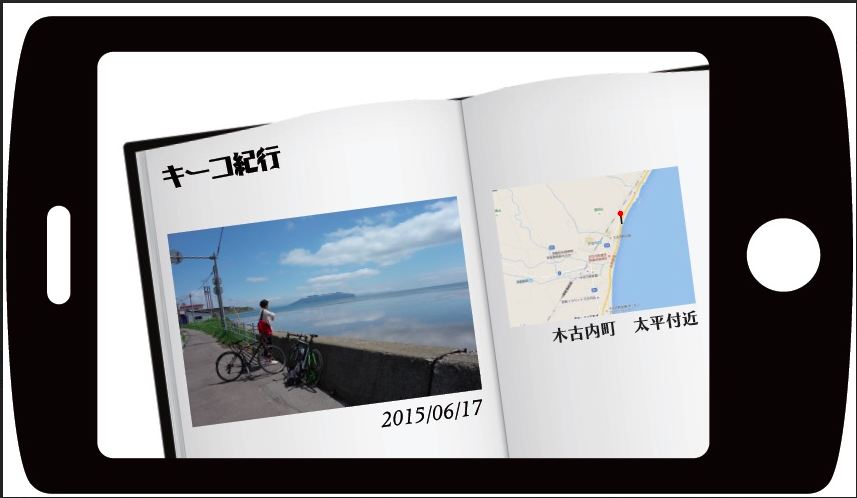
\includegraphics[width=9cm, bb=0 0 857 498]{5.1_kikou.png}
 \end{center}
 \caption{紀行の画面イメージ}
 \label{fig:one}
\end{figure}

\section{第一回アプリ提案}
6月半ば時点での提案アプリは、マップ上に表示された観光スポットをタップすると簡易情報を吹き出しで表示し、その吹き出しをタップすると詳細情報が掲載されたWebページへ画面が遷移するというものであった。この他には、木古内町民しか知らないニュースや木古内町の天気をマップ画面右上に表示する機能や、ユーザ同士で木古内町内の写真を共有できる機能、木古内観光協会が公開している木古内お散歩コースをマップの中に盛り込む機能を考案していた。この時点ではアプリの実装を行っておらず、画面のイメージ案のみ作成していた。考案した機能のうち、画面イメージを作成出来たのは、マップ画面、Web ページを表示する画面、お散歩コースを表示する画面の3 つである。6月12日に行った外部講師とのテレビ会議でこの提案に対するレビューを受けた結果、現在の提案に木古内らしさを加える必要があるとの指摘を受けた。

\bunseki{岩見建汰}


\begin{figure}[htbp]
  \begin{center}
    \begin{tabular}{c}

      % 1
      \begin{minipage}{0.33\hsize}
        \begin{center}
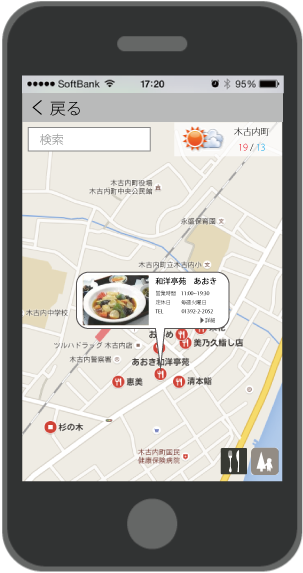
\includegraphics[width=4cm, bb=0 0 303 573]{5.2_map1.png}
          \hspace{1cm} [1]観光スポットの紹介
        \end{center}
      \end{minipage}

      % 2
      \begin{minipage}{0.33\hsize}
        \begin{center}
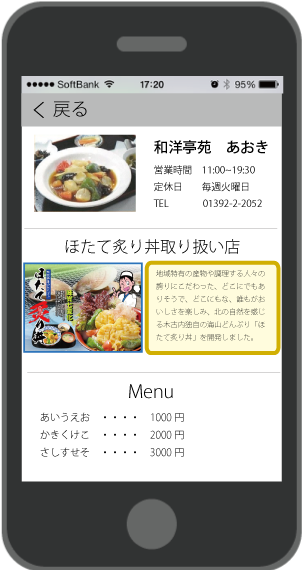
\includegraphics[width=4cm, bb=0 0 304 570]{5.2_map2.png}
          \hspace{1cm} [2]観光スポットの詳細情報
        \end{center}
      \end{minipage}

      % 3
      \begin{minipage}{0.33\hsize}
        \begin{center}
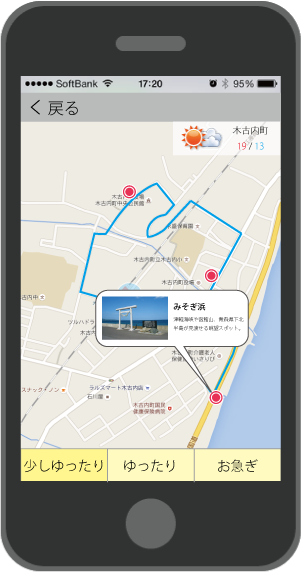
\includegraphics[width=4cm, bb=0 0 302 572]{5.2_sanpo.png}
          \hspace{1cm} [3]お散歩コース
        \end{center}
      \end{minipage}

    \end{tabular}
    \caption{初期段階での画面イメージ}
    \label{fig:lena}
  \end{center}
\end{figure}

\section{第二回アプリ提案}
ここで記述するver.1.0 とは、観光スポットを紹介する機能と天気を表示する機能を含んだアプ
リのことだ。前者の機能は4 章でも記述している勉強会で取り扱った、マップに関する技術とテキストファイルから情報を取り込む技術の2 つを応用させて実現した。また、天気を表示する機能についてはJSON データを用いて木古内町の現在、3 時間ごと、向こう1週間の天気を表示する機能を実装した。以下に示す図5.3 はver.1.0 で完成していた画面だ。その後は、初期段階で実装する予定だったニュースは、継続運用を考えるとニュースの更新が難しいという理由で保留にした。さらに、お散歩コースをマップの中に盛り込む機能は公開されていたコース内容が車での移動を前提にしており、自分たちでコースを作らなければいけないということになり実装は保留となった。また、ポスターのレビューの際にアプリの機能についてユーザストーリーに問題があるとの指摘を受けた。具体的には、観光客は観光スポットやランドマークの写真を見てからその場所へ行くのが通常の流れである。しかし、当時作成していたver.1.0 は場所を伝えてから写真や詳細情報を見せる流れになってしまっていた。この状態だと木古内町の魅力はもちろんのこと、何があるかすら伝わらないとの内容であった。この指摘を受けてver.2.0 を開発することに決定し、カスタマージャーニーマップを用いてユーザストーリーの再考を行った。

\bunseki{岩見建汰}


\begin{figure}[htbp]
  \begin{center}
    \begin{tabular}{c}

      % 1
      \begin{minipage}{0.33\hsize}
        \begin{center}
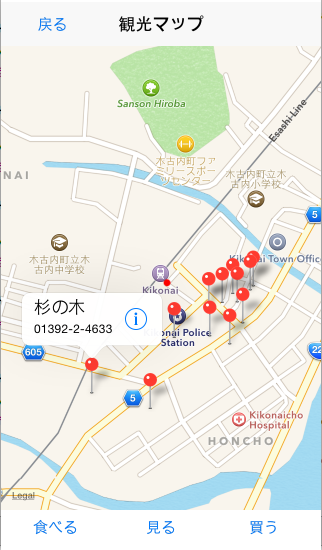
\includegraphics[width=4cm, bb=0 0 322 550]{5.3_map1.png}
          \hspace{1cm} [1]観光スポットの紹介
        \end{center}
      \end{minipage}

      % 2
      \begin{minipage}{0.33\hsize}
        \begin{center}
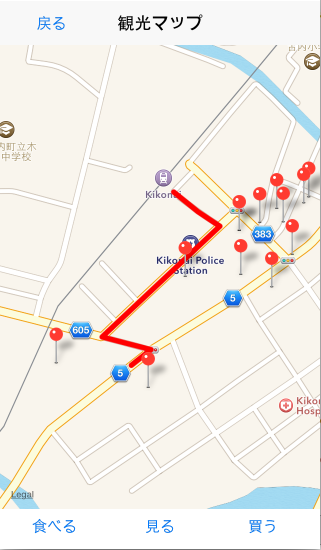
\includegraphics[width=4cm, bb=0 0 321 550]{5.3_map2.png}
          \hspace{1cm} [2]ルート案内
        \end{center}
      \end{minipage}

      % 3
      \begin{minipage}{0.33\hsize}
        \begin{center}
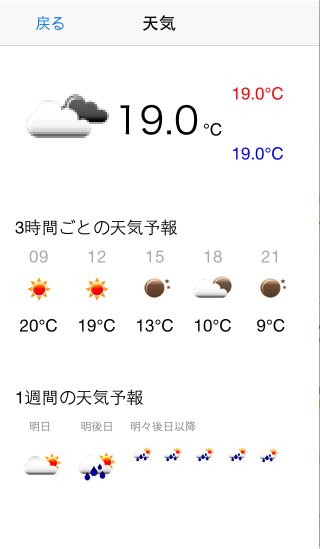
\includegraphics[width=4cm, bb=0 0 320 549]{5.3_weather.png}
          \hspace{1cm} [3]木古内町の天気を表示
        \end{center}
      \end{minipage}

    \end{tabular}
    \caption{ver.1.0の完成画面}
    \label{fig:lena}
  \end{center}
\end{figure}

\section{中間発表}
ここで記述するver.2.0 とは、ver.1.0 で指摘を受けたユーザストーリーを考慮した挙動へと修正
した機能が実装されているアプリのことだ。中間成果発表会まで残り1 週間を切っていたため新たな機能を追加して修正するのは間に合わないと判断し、ver.1.0 で実装していた部分の情報の見せ方を改善する方針で議論を進めた。主な内容として、以前はカテゴリ別にピンを表示していたがピンではなく写真を表示するように仕様を変更した。また、お店の詳細情報としてWeb ページを表示する内容だったが、お店のメニュー表や営業時間などの情報を我々で作成した画面構成を用いることにした。図5.4[2] の右上にあるMap の文字をタップすると、現在地からお店までのルートをマップで表示する仕様に変更した。以下に示す図5.4 はver.2.0で完成していた画面だ。
中間成果発表会では木古内町の歴史に関する情報を表示する機能が欲しいとの意見をもらった。また、図1.1 に示してあるフォトストーリーの画面案に関して1 つの画面に写真が2 枚もあると分かりにくいのではという意見ももらった。
\bunseki{岩見建汰}

\begin{figure}[htbp]
  \begin{center}
    \begin{tabular}{c}

      % 1
      \begin{minipage}{0.33\hsize}
        \begin{center}
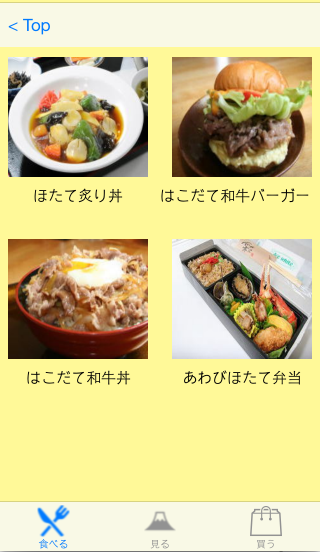
\includegraphics[width=4cm, bb=0 0 320 552]{5.4_category.png}
          \hspace{1cm} [1]観光スポットの紹介
        \end{center}
      \end{minipage}

      % 2
      \begin{minipage}{0.33\hsize}
        \begin{center}
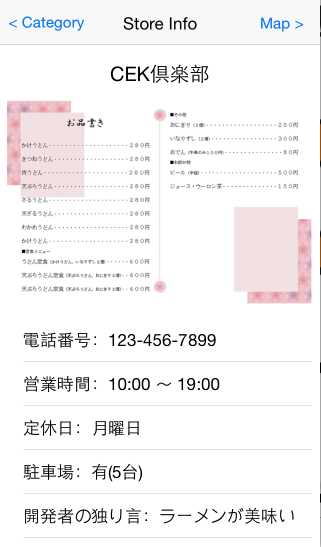
\includegraphics[width=4cm, bb=0 0 321 547]{5.4_detail.png}
          \hspace{1cm} [2]ルート案内
        \end{center}
      \end{minipage}

      % 3
      \begin{minipage}{0.33\hsize}
        \begin{center}
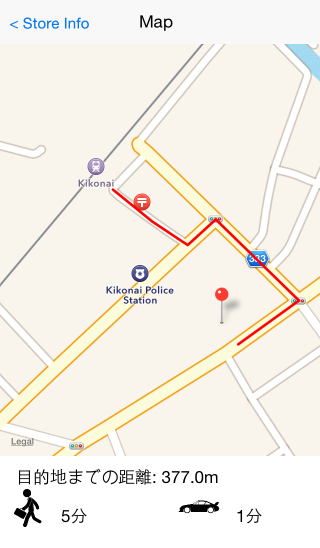
\includegraphics[width=4cm, bb=0 0 320 548]{5.4_route.png}
          \hspace{1cm} [3]木古内町の天気を表示
        \end{center}
      \end{minipage}

    \end{tabular}
    \caption{ver.2.0の完成画面}
    \label{fig:lena}
  \end{center}
\end{figure}


%に
\chapter{結果}
本プロジェクトの目的は、木古内町への観光客の満足度を高めることである。前期の活動では、木古内町の魅力である観光地や食べ物、お土産などの情報を発信する機能を作成した。これにより、木古内町の特色を知らない観光客に、どのようにして木古内町の魅力を発信するかという方法を提案することはできた。しかし、実際のお店や観光地などの木古内町の情報を集め、アプリに掲載するところまでは前期中の活動ではできなかった。よって、木古内町の観光情報が分散し、そのアクセス性が低いという問題の解決はまだ完全にはできていない。また、観光で得られる体験に付加価値を与える機能としてフォトストーリーを考えているが、どのようにして利用者の紀行をつくるのか、具体的にどのようなものが作成されるのかという詳細な機能についてはまだ決まっていない。本プロジェクトの目標は、木古内町へのフィールドワークで得られた経験から、アプリケーションを設計し、開発言語であるSwiftを学びながらアジャイル開発を行うというものだった。前期の活動では、Git や Swift などの開発方法を勉強会を通して学び、アジャイル手法を用いて前期中に 2 度のアプリケーション開発を行った。しかし、木古内町でのフィールドワークで得られた経験に基づいた、木古内町の特色を活かした機能はまだ提案できていない。よって、開発の知識に関しての学びは多かったが、フィールドから得られたことを開発にはまだ生かし切れていない。

\bunseki{池田俊輝}


\chapter{今後の課題と展望}
後期の活動としては、現在は分散している観光情報を全て取得できていないので、木古内をより調査する必要がある。調査方法としては、再度木古内にフィールドワークを行うことと、木古内町が提供している観光情報をより調査することを想定している。また、開発中のフォトストーリーの機能の詳細を決め実装する予定だ。フォトストーリーをユーザが作成するにあたり、いかにユーザに負担をかけないようにするかが課題になる。また、写真から撮影した観光地の現在地を取得し、その場所の観光情報を表示する予定だが、本当に可能なのか調べる必要がある。その後、道南いさりび鉄道の従業員の方などの木古内関係者に実装したアプリをレビューしてもらい、新たなアプリの機能案を検討する方針である。

\bunseki{池田俊輝}

\chapter{まとめ}
 本プロジェクトの目的は、木古内町への観光客の満足度を高めることである。そのために、観光情報へのアクセス性を高めること、観光で得られる体験に付加価値を与えることを実現する機能をもつアプリの開発を行う。前期中の活動では、観光情報のアクセス性向上を目指す機能を実装したが、アクセス性を高めるという課題はまだ完全には解決できていない。また、観光体験に付加価値を与える機能として旅行の記録を作るフォトストーリーを考えているが、どのように、どのような記録が作られるのかといった詳細な機能については未定である。後期の活動としては、現在は分散している観光情報を我々も把握できていないため、木古内をより調査する必要がある。また、フォトストーリーの詳細な仕様を決定し実装する予定である。その後、実装したアプリをレビューしてもらい、新たなアプリの機能案を検討する方針である。
\bunseki{細川椋太}

% 以降、付録(付属資料)であることを示す
\begin{appendix}
\chapter{新規習得技術}
\section{アジャイル開発手法/スクラム}
アジャイル開発とは、ソフトウェアを迅速に、かつ現場のニーズに応えながら開発することである。本プロジェクトはフィールドからのフィードバックを取り入れながらアプリケーションの開発を行うことを目標としている。したがって、ウォーターフォールモデル等、長期的な計画に基づいて1バージョンを開発する方式ではこの目標を十分に達成し得ない。アジャイル開発によって短い期間での開発と評価を繰り返し、その度にフィールドからのフィードバックを反映していくことがこのプロジェクトの意義である。アジャイル開発とは同様の理念で開発を進める手法の総称であるが、本プロジェクトではこのうちスクラムについて理解を深め、実践していくことを目指すものである。本プロジェクトを通して実践した内容については3.2.1を参照されたい。この節では主にスクラムに関連する用語について述べてゆく。\par
スクラムにおいて、優先度順のタスクリストはバックログと呼ばれる。そのうち、当該バージョンを開発するにあたってのタスクをすべて記述したものをプロダクトバックログという。このプロダクトバックログをタイムボックス、すなわち定められた一定期間ごとに分割したものをスプリントバックログといい、それぞれのタイムボックスをスプリントという。スプリントは通常1週間から4週間の期間が設定されることが通例である。本プロジェクトでの実践もこれに則り、3.2.1で述べたように1つのスプリントは1週間としている。スプリントバックログを作成する際には、チームメンバが確実に消化しきれるタスク量とするほか、スプリント終了時に動くソフトウェアが存在していることが重要である。つまり、スプリントバックログを消化した時点でマイナーバージョンが、プロダクトバックログを消化した時点でメジャーバージョンがリリースされることとなる。各スプリント期間中は、毎日決められた時間にミーティングを行う。これをスクラム会議といい、「前回の会議以降の作業報告」「次回の会議までの作業計画」「作業上の問題点の報告」を各メンバーが報告し、認識を共有する。この会議は15分以内で終わらせるべきとされており、重大な案件に関しては会議終了後個別に行われることとなる。このように、短期的な計画に基づく実装と、メンバ間の認識の共有を重視する点がスクラムの特徴である。
\bunseki{横山翔栄}


\section{WebAPI}
アプリケーションの作成にあたり、天気の情報を取得するためにWebAPIを利用した。これはHTTP等のWeb技術を用いてプログラムの提供する機能を利用するためのサービスであり、有償のものも含め多くの種類が公開されている。本プロジェクトの成果物には``OpenWeatherMap''\footnote{http://openweathermap.org/}を利用しており、このAPIから返されるJSON形式のデータを処理することで、天気情報を表示している。WebAPIの優れている点は、インターネットに接続された環境であればどこからでも利用できるという点である。前述の通り、WebAPIはHTTPなどのWeb技術を用いたサービスである。このため、特殊な機器やシステムを一切使用することなく、多くの機器で普遍的に利用することができる。
\bunseki{横山翔栄}

\section{Swift/Xcode}
開発言語には 4.1 でも記述している通り Swift を用いることとした。Swift を使ったアプリを開発するために参考文献に記してある「Swift ではじめる iPhone アプリ開発の教科書」を用いた。この本では基本的な制御文やスクロールバーやスイッチの使い方などを習得した。地図アプリを作成するにあたってはマップの表示、ピンの動作などの基礎部分を勉強会で習得し、その後はインターネットでコード例がないか調べて勉強会の内容を応用させた。また、一般的にはマップ上に表示されている物体をピンと呼んでいるが内部的にはアノテーションと呼ぶ。このアノテーションをクラス化して配列で管理することにより、複数のピンを同時に表示させた。Xocdeについては勉強会で新規プロジェクトを作成する方法からエラーの見方や各種アイテムの配置方法を学んだ。
\bunseki{岩見建汰}

\section{Git/GitHub}
この節では、Git/GitHubを使うにあたり重要となる用語や概念について述べていく。Git/GitHubは分散型バージョン管理システムと呼ばれ、ファイルの変更履歴を管理するシステムである。変更履歴がソースコード等のファイルとは別ファイルで管理されているため、誤って変更してしまったファイルを前の状態に戻すことができる。また、Git/GitHubはファイルの一貫性も保持する仕組みになっている。上記で説明した変更履歴やソースコード等のファイルはリポジトリと呼ばれる場所に保存されている。リポジトリからコピーしたファイルに変更を加えて、リポジトリに変更したファイルを保存することをコミットと呼ぶ。チームで開発をする際にこのコミットが
たくさん行われたり同時に作業を進めることがある。その結果、変更履歴の管理が複雑になってしまい混乱する問題が起きる。その問題を解決するのがブランチと呼ばれるものである。ブランチは変更履歴の流れを分岐していくものであり、別々の作業を他人の作業に干渉することなく進めることができる技術である。このブランチの中でも常に動くソフトウェアが反映されるべきブランチをmasterブランチと呼ぶ。以下にGit/GitHubを用いたアプリ開発の具体的な流れを示す。
\begin{enumerate}
 \item リモートリポジトリにあるファイルをローカルにコピーする。
 \item masterブランチからdevelopブランチを作成する。
 \item 新規作成したブランチにリモートブランチの内容を取り込む。
 \item 取り込んだファイルを変更する。
 \item 変更したファイルをステージする。
 \item 変更内容をコミットする。
 \item コミットした内容をリモートリポジトリに反映させる。
\end{enumerate}

\bunseki{岩見建汰}

\chapter{活用した講義}
 報告書の参考文献を明示するために、科学技術リテラシーで学んだ参考文献の書き方の知識を用いた。、また、中間発表で用いたポスターを作成するにあたって、情報表現基礎や情報デザインの講義で得た知識や経験を用いた。見やすく分かりやすいポスターを作るために、できる限り文字を図にして置き換え、図解によって主要を伝えるという点を意識した。また、全体の印象を整えるため各要素の位置を他の要素にそろえた。プロジェクトを進めていくうえでアプリの開発形態を見直すとき、ソフトウェア設計論I  で学んだウォーターフォールモデルとアジャイル開発手法の考え方を参考にした。本プロジェクトはアジャイル開発手法であり、ウォーターフォールモデルのような1つ1つの段階を固めてから次の段階に進むということはせず、開発を迅速に行いレビューを受け、再び開発をしていくものであるということを常に意識することが重要だと学んだ。アプリはどのような機能を持っているか、ユーザはどのようにアプリを使うのかを明示してそれを設計するためにソフトウェア設計論II  のユースケース図とアクティビティ図の書き方を参考にした。以下が作成した図である。

\bunseki{山川拓也}

    \begin{figure}{}
        \begin{center}
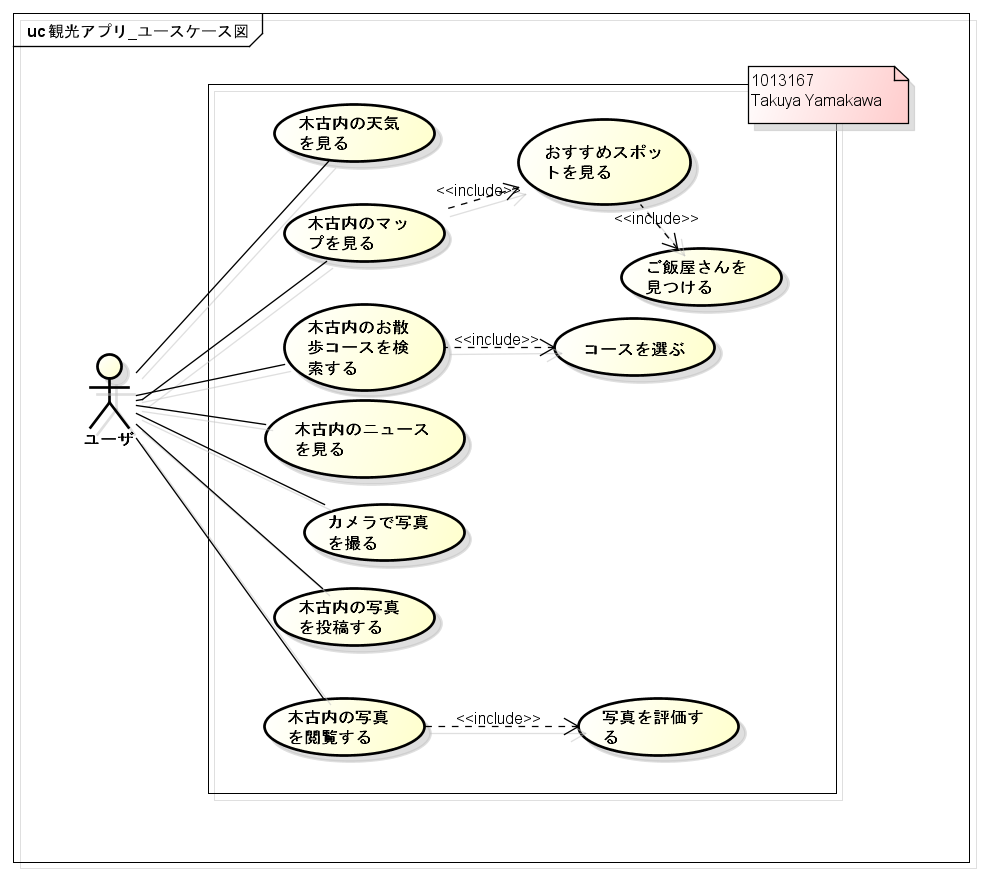
\includegraphics[width=14cm, bb=0 0 520 388]{project_usecase2.png}
        \end{center}
         \caption{ユースケース図}
 \label{fig:one}
      \end{figure}
 

    \begin{figure}{}
        \begin{center}
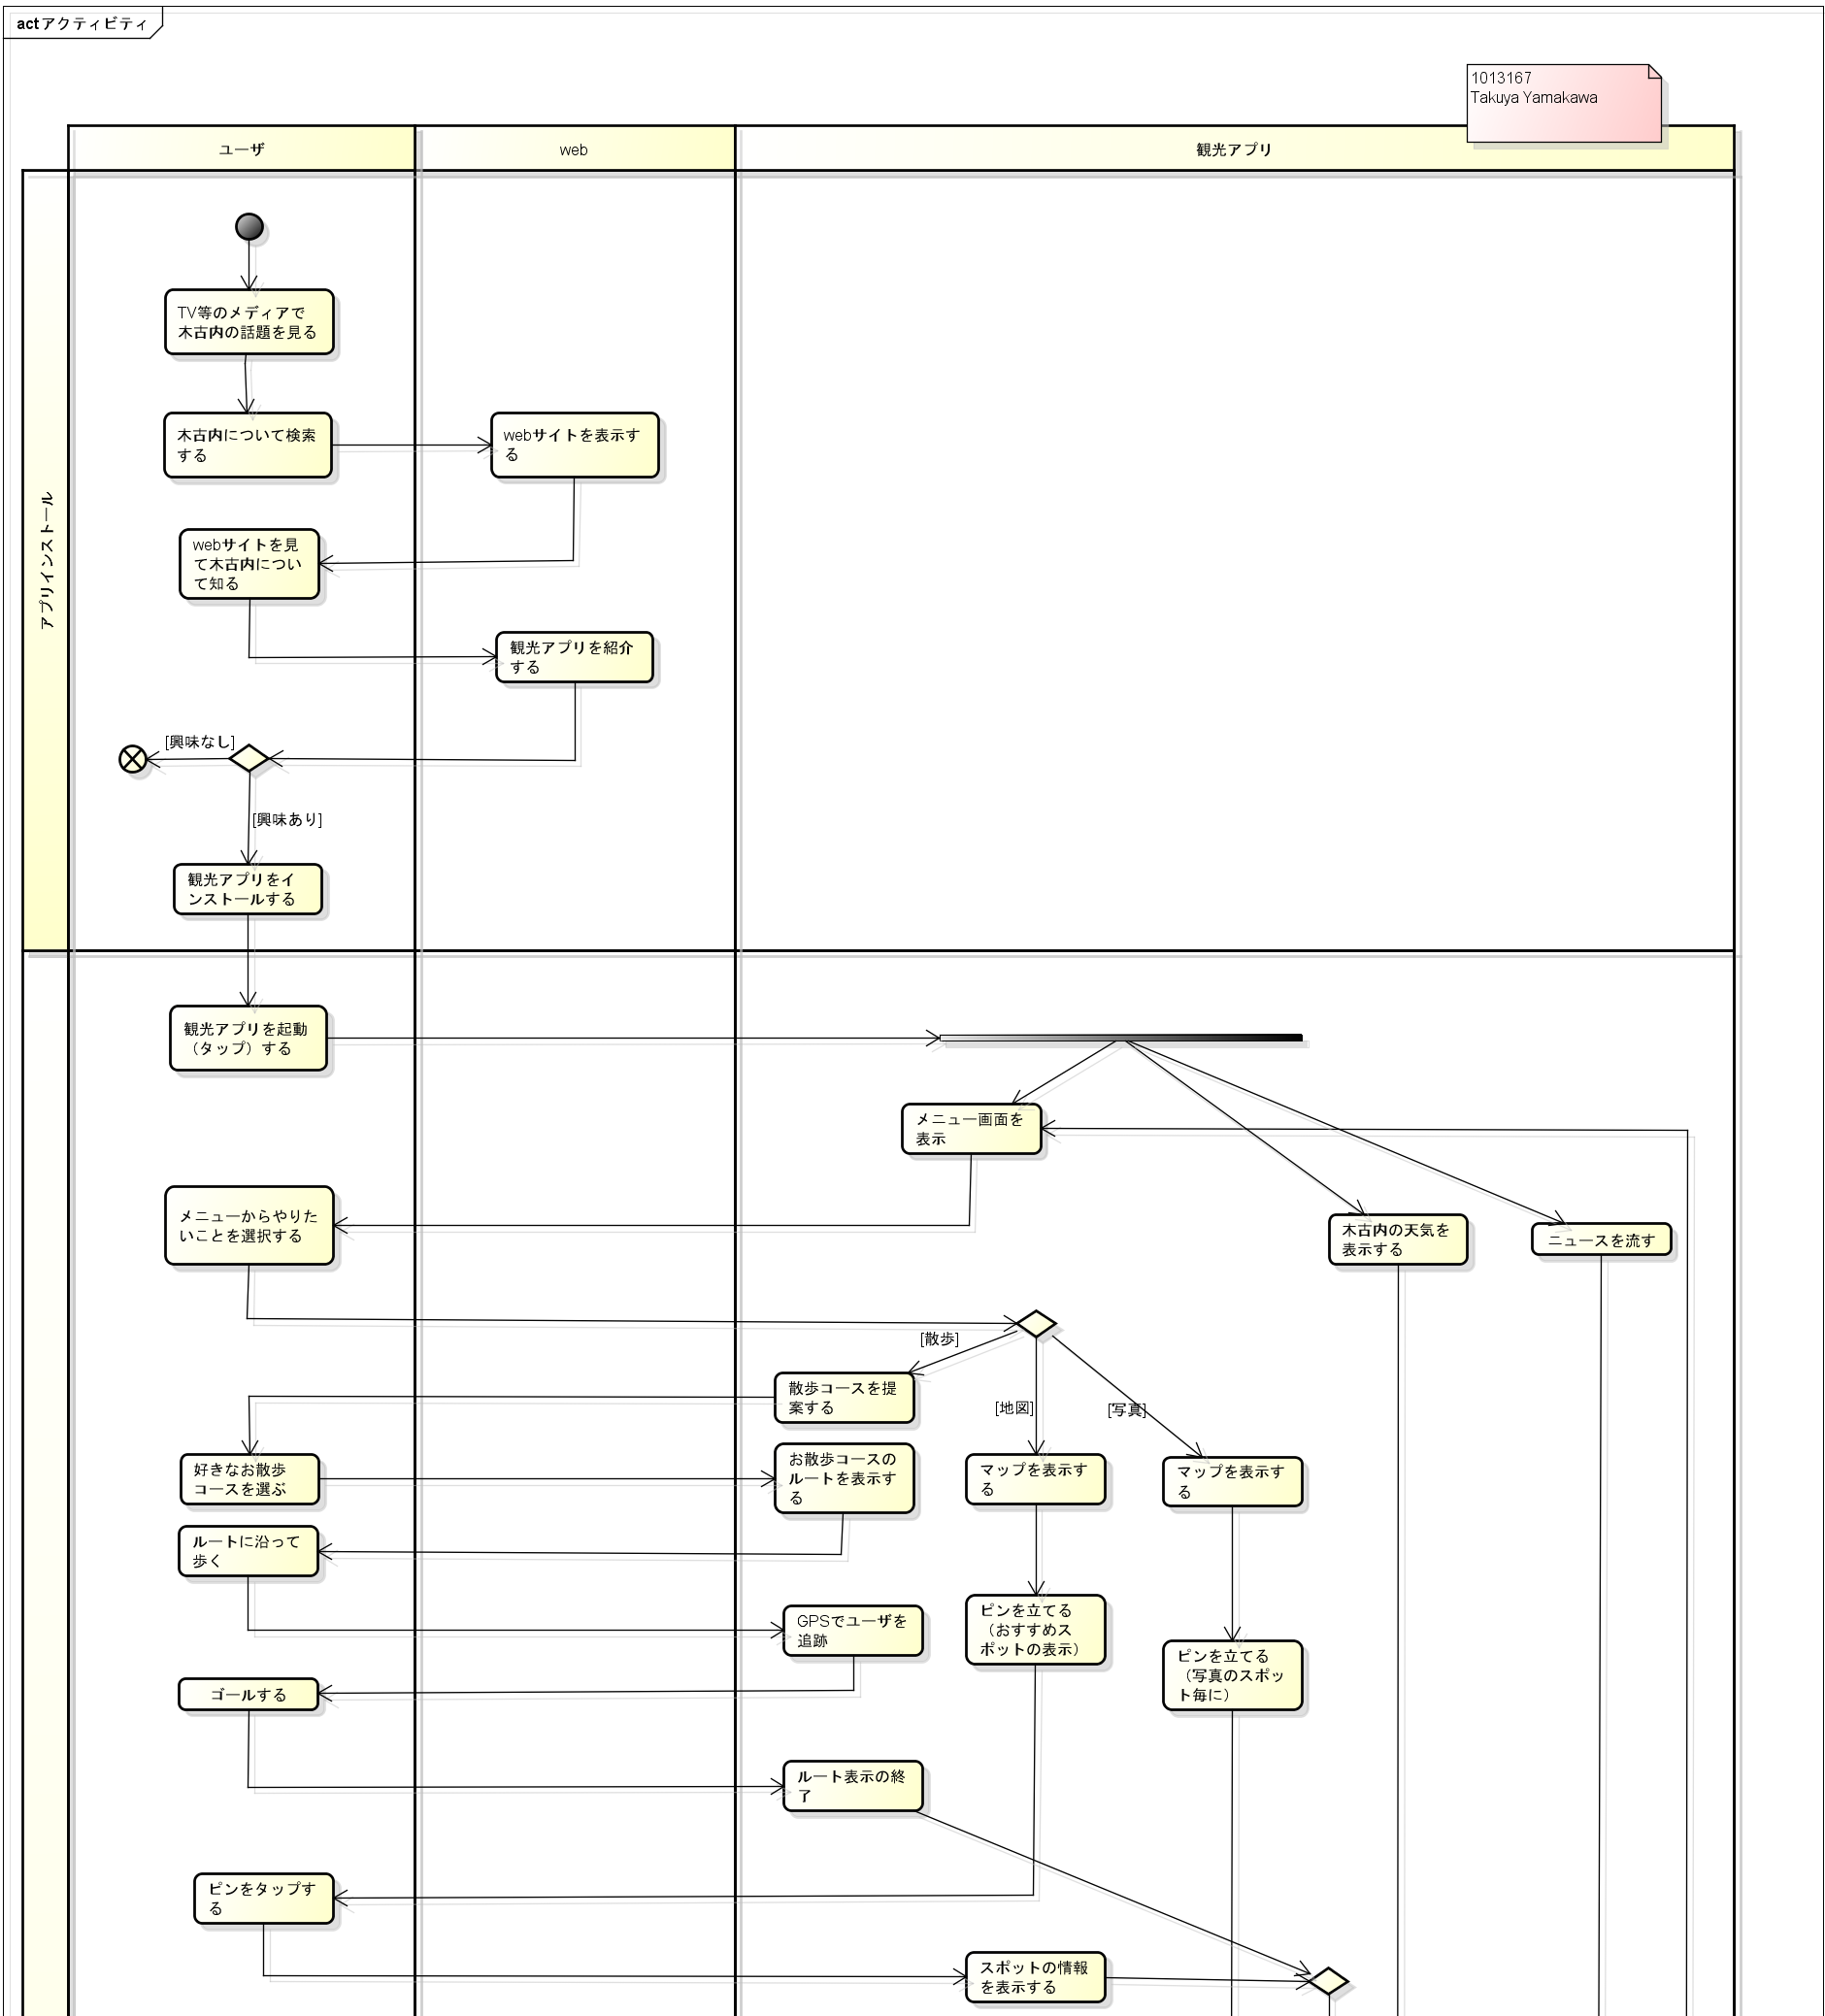
\includegraphics[width=20cm, bb=0 0 1880 2077]{project_activity2.2-1.png}
        \end{center}
 \label{fig:one}
      \end{figure}
      

       \begin{figure}{}
        \begin{center}
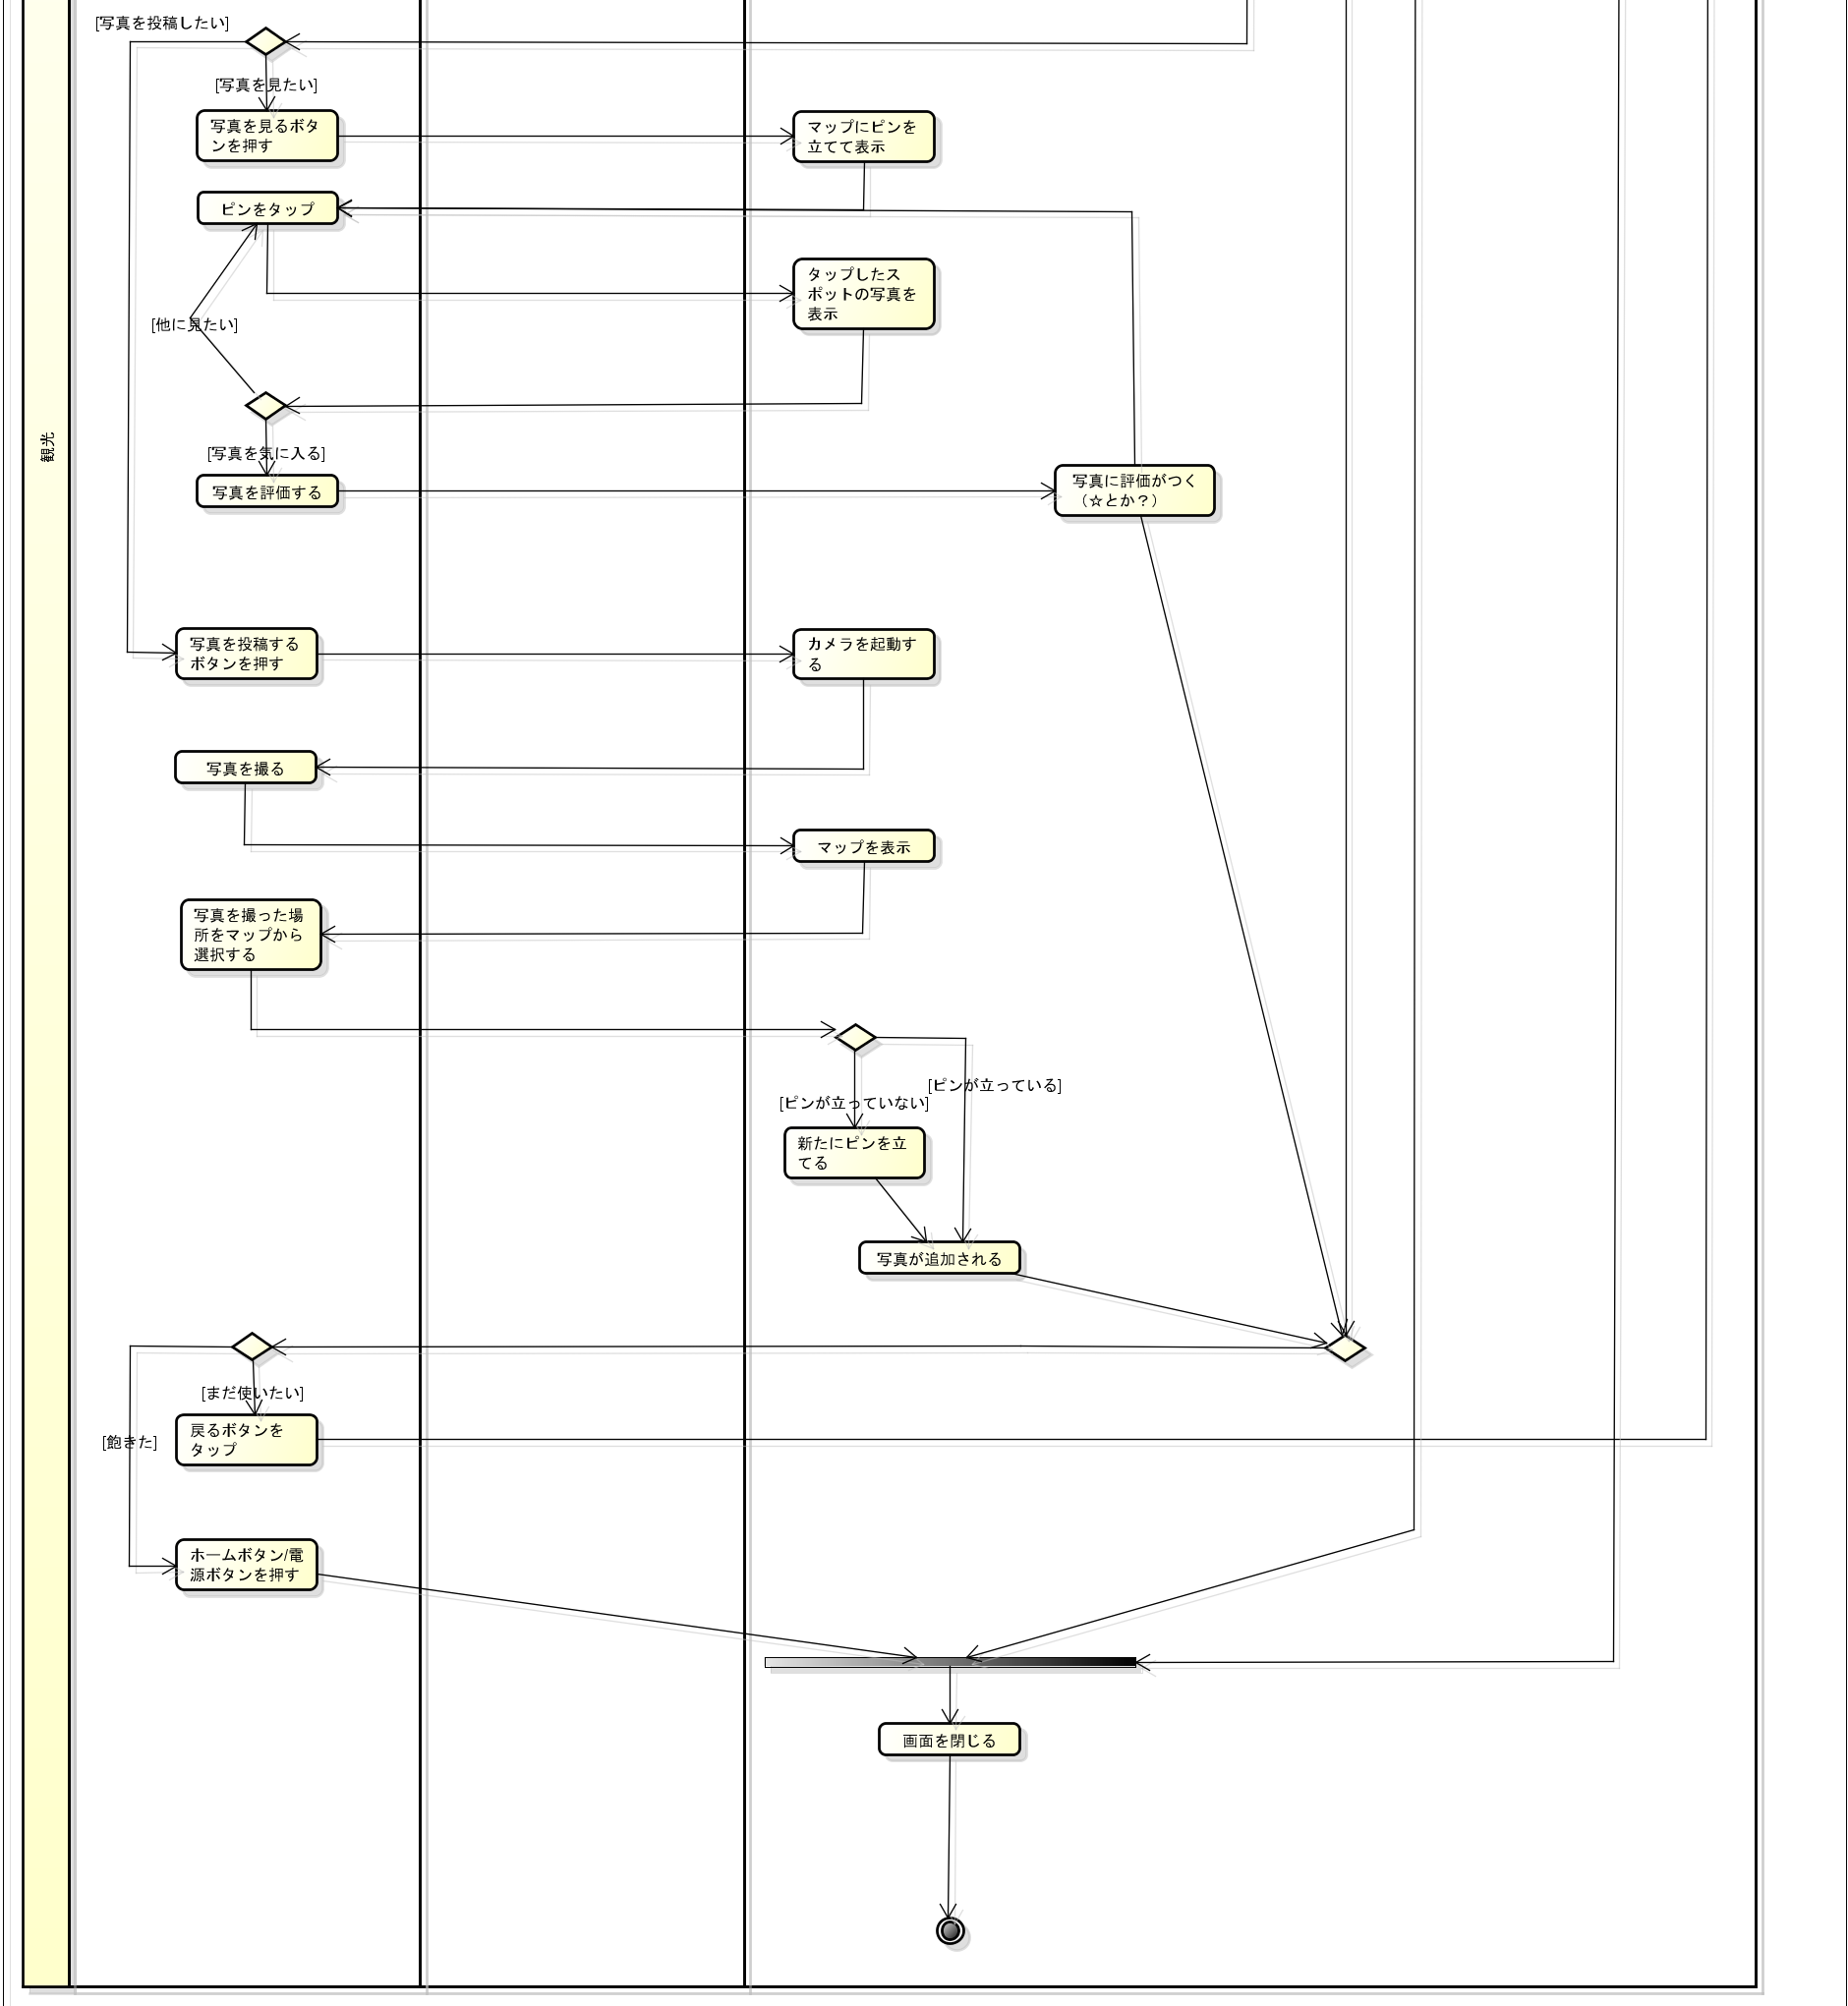
\includegraphics[width=20cm, bb=0 0 1880 2041]{project_activity2.2-2.png}
        \end{center}
                 \caption{アクティビティ図}
 \label{fig:one}
      \end{figure}   
      

%付録の終わり
\end{appendix}


%\backmatter

% 参考文献
\begin{thebibliography}{9}
\bibitem{NN2013}
\newblock 西村直人,永瀬美穂,吉羽龍太郎
\newblock SCRUM BOOT CAMP THE BOOK.
\newblock 株式会社翔泳社, 2013.

\bibitem{YM2014}
\newblock 森巧尚.
\newblock Swift ではじめるiPhone アプリ開発の教科書.
\newblock 株式会社マイナビ, 2014.

\bibitem{HO2014}
\newblock 大塚弘記.
\newblock WEB+DB PRESS plusシリーズ GitHub実践入門 -Pull Requestによる開発の変革.
\newblock 株式会社技術評論社, 2014.

\bibitem{HH1980}
佐賀市南部周遊バスで行く SAGAARIAKEガタバトルコース. 佐賀市. \par
http://www.saga-city.jp/gatabattle/tour.html. (2015/7/22 アクセス)

\bibitem{YI2003}
いさりび鉄道に事業許可 国交省 来春開業へ準備本格化. どうしんウェブ/電子版, 2015.\par
http://dd.hokkaido-np.co.jp/news/politics/politics/1-0151087.html. (2015/7/22 アクセス)

\bibitem{KI1989}
北海道情報誌 HO[ほ] バックナンバー. 株式会社 ぶらんとマガジン社, 2015.\par 
http://www.toho-ho.jp/backnumber. (2015/7/22 アクセス)

\bibitem{TK1995}
デザインの「まとめる」を、ちょびっとかじる。.  	アトリエ・カプリス. \par
http://dzukai.com/egokoro/ws\_matome\_ex.html. (2015/7/22 アクセス)

\bibitem{TK1993}
Japan - The Strange Country (Japanese ver.). vimeo.com, 2010.\par
https://vimeo.com/9873910. (2015/7/22 アクセス)

\bibitem{KK2004}
統計データを「心に響く動画」に変える”ビデオインフォグラフィック”とは?. movieTIMES, 2014.\par
http://www.movie-times.tv/purpose/branding\_idea/4366/. (2015/7/22 アクセス)

\bibitem{NK1994}
クールなインフォグラフィック動画15選. HepHep!, 2013.\par
http://hep.eiz.jp/201306/infographics/. (2015/7/22 アクセス)

\bibitem{NM1998}
木古内町で記念事業続々道新150604.pdf. 北海道新聞, 2015.\par
https://www.dropbox.com/s/juxgayyd1y7h3eu/%E6%9C%A8%E5%8F%A4%E5%86%85%E7%94%BA%E3%81%A7%E8%A8%98%E5%BF%B5%E4%BA%8B%E6%A5%AD%E7%B6%9A%E3%80%85_%E9%81%93%E6%96%B0150604.pdf?dl=0
. 
(2015/7/22 アクセス)

\bibitem{SN1991}
日曜トーク道新150531.pdf. 北海道新聞, 2015.\par
https://www.dropbox.com/s/ic7ew6fvxospnp9/%E6%97%A5%E6%9B%9C%E3%83%88%E3%83%BC%E3%82%AF_%E9%81%93%E6%96%B0150531.pdf?dl=0
. (2015/7/22 アクセス)

\bibitem{NO2000}
5分で分かる、「スクラム」の基本まとめ. atmarkIT, 2012.\par
http://www.atmarkit.co.jp/ait/articles/1208/07/news128.html. (2015/7/22 アクセス)

\bibitem{CQ1991}
町長がメールで木古内PR. 函館新聞, 2015.\par
http://www.hokkaido-nl.jp/detail.cgi?id=26392. (2015/7/22 アクセス)

\bibitem{IS1991}
Swiftで写真からGPS情報を取得. psychosistem.jp, 2014.\par
http://psychosistem.jp/blog/?p=934. (2015/7/22 アクセス)

\bibitem{}
Googleマップで緯度経度を求める. numazu-ct.ac.jp.\par
http://user.numazu-ct.ac.jp/-tsato/webmap/sphere/coordinates/advanced.html. (2015/7/22 アクセス)

\bibitem{}
SwiftでAppDelegateを使った画面間のデータ受け渡し. Qiita.com, 2014.\par 
http://qiita.com/xa\_un/items/814a5cd4472674640f58. (2015/7/22 アクセス)

\bibitem{}
アノテーションに画像を追加. SwiftDocs, 2015. \par
https://sites.google.com/a/gclue.jp/swift-docs/ni-yinki100-ios/7-mapkit/anoteshonni-hua-xiangwo-zhui-jia. (2015/7/22 アクセス)

\bibitem{}
Swiftコードで画面遷移させたいときの方法. cheekpouch.com, 2014.\par
http://blog.cheekpouch.com/352/. (2015/7/22 アクセス)

\bibitem{}
実践! iPhoneアプリ開発. マイナビニュース, 2009.\par
http://news.mynavi.jp/column/iphone/017/. (2015/7/22 アクセス)

\bibitem{}
木古内町観光協会. 木古内町.\par
http://kikonai-kankou.net/. (2015/7/22 アクセス)
\end{thebibliography}

\end{document}